\documentclass[12pt,a4paper,twoside]{report}

\usepackage[pdfborder={0 0 0}]{hyperref}

\usepackage[margin=25mm]{geometry}

\usepackage{graphicx}
\graphicspath{ {images/} }


\usepackage{parskip}

%!TeX spellcheck = en-UK

\begin{document}

% Main document TODO: Cover Page, Proforma Page, Decleration of Originality and
% Table of contents

{\large

\begin{tabular}{ll}

Name:               & \bf Tom Read-Cutting, \href{mailto:tr395@am.ac.uk}{\nolinkurl{tr395@cam.ac.uk}}  \\

Project Title:      & \bf  \normalsize{Simulating Wavefronts in Real-Time using Wave
Particles \\

Supervisor:         & \bf Dr Rafal Mantiuk                    \\

Director of Studies:        & \bf Dr R.~K.~Harle  \\

Overseers:         & \bf Prof L.~Paulson  \& Dr I.~J.~Wassel \\

\end{tabular}

}

In brief, the goal of my Part II project is to implement a real time water wave
simulation technique called Wave Particles, that captures how wavefronts form
and propagate by representing them as particles on a 2D plane.
Applications such as complex video games and virtual reality experiences
frequently use innacurate real-time approximations of physical systems.
Therefore I made it my goal to implement this system within the Unity game
engine.

\begin{figure}[h]
\centering
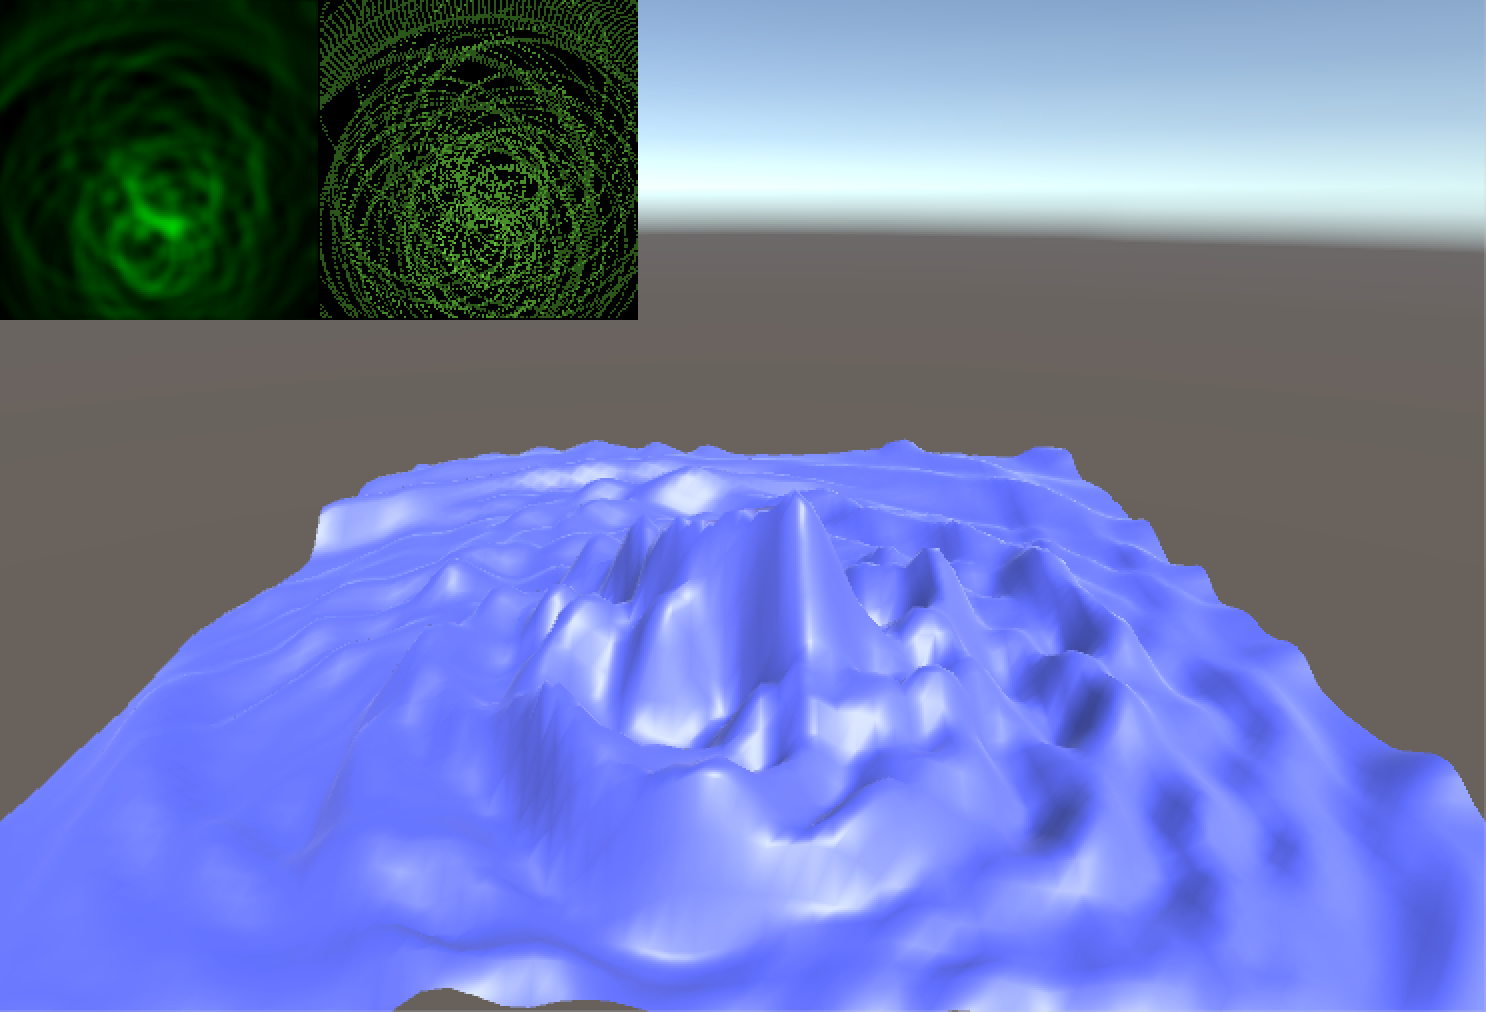
\includegraphics[width=0.8\textwidth]{wave_particles_gpu}
\caption{\textit{Succesfully convolving wave particles on the GPU. The top-left box in
the image shows the Wave Particles texture, while the one next to it shows the
position of Wave Particles on the plane.}}
\end{figure}

Sticking to schedule, I made effective use of the first two weeks to gain a
thorough understanding of the paper on Wave Particles and additional material in
the field of fluid simulation and real-time systems.

The next task I engaged in was learning the Unity game engine and graphics
programming as I had never done either before. The scripting language used by
Unity, C\# is very similar to Java which I am experienced in, so the focus of
learning was Unity's APIs, working with the creation tools, and shader
programming. As Unity is so complex, getting the initial foothold that got me
started was rather difficult, and for the first month everything required
various attempts to get right. I also realised that achieving some my goals
out-of the order I had planned would be best, as I gained a better understanding
of all the systems involved. A good example of this was the initial intention to
implement everything on the CPU before porting everything to the GPU. As each
component of the Wave Particles system are individually complex on the CPU, it
ended up making sense to incrementally implement components on the GPU before
moving onto the next one on the CPU. The slowdown handling every system together
on the CPU, would have been a major burden on viewing the results and iteration
times.

For this reason I have yet to completely implement fluid-object interaction, but
am slightly ahead of schedule on porting code to the GPU. One major issue worth
mentioning, was a mistake made in attempting to port Wave Particle convolution
to the GPU which led to the issue shown in Figure \ref{fig:fail}.

\begin{figure}[h]
\centering
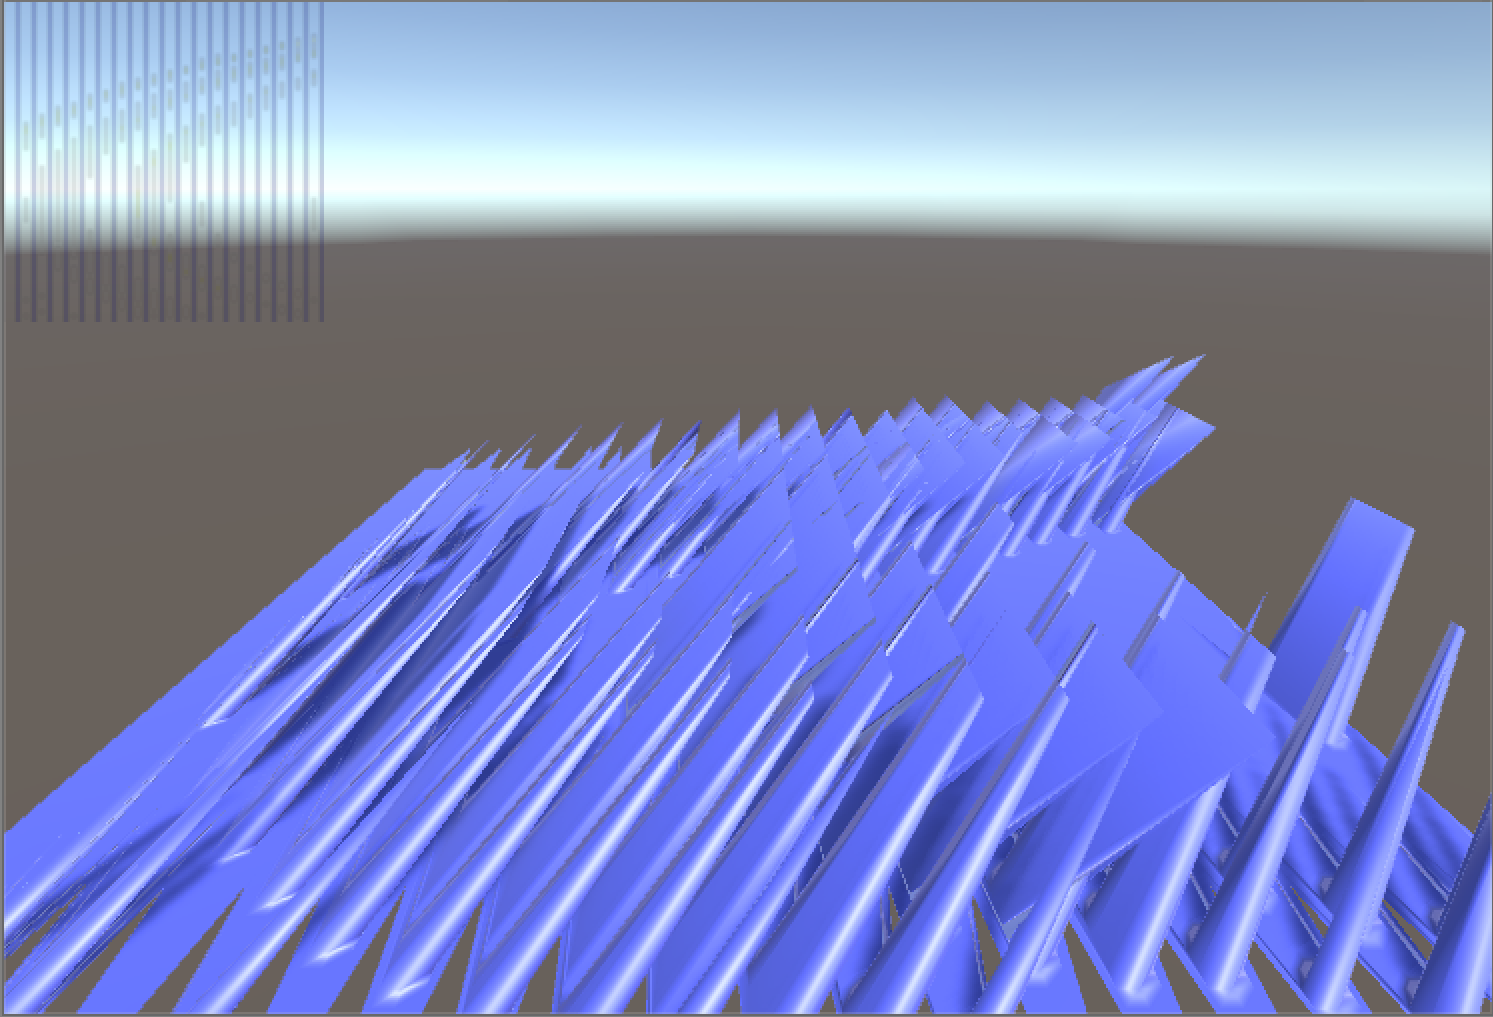
\includegraphics[width=0.8\textwidth]{texture_copy_issues}
\caption{\textit{The first attempt at Texture convolution on the GPU.}}
\label{fig:fail}
\end{figure}

This was because I had accidentally set one of the textures involved to the
ARGB32 format, as opposed to the intended RGBAFLOAT format. However, as the
other textures were all set to the correct format, copying from one to the other
caused incompatability major issues! The problem being that Unity didn't
complain about this obvious error. It took 4 sets of eyes and 3 weeks for this
one issue to be resolved (other aspects of the system were worked on in the mean
time, but this one issue did cause some slowdown!).

To conclude, most of my schedule has been achieved, including being further
ahead in some aspects. I have written a first-draft of the introduction of my
dissertation and implemented the core of the Wave Particles system on the CPU in
addition to some aspects on the GPU. Whilst tying everything into the Unity Game
Engine. However, I have reshuffled some aspects of my timetable, such as when
fluid-object interaction should be completed, now being the 20th of February.
Therefore, I would estimate that I am approximately a week behind in what I
aimed to achieve, but progress has accelerated significantly in the past month.
Despite some of the hurdles faced, my original schedule has provided enough
flexibility to handle them and I am not concerned about hitting my targets in
the coming weeks.

\end{document}
